\documentclass[a4paper]{article}

%% Language and font encodings
\usepackage[english]{babel}
\usepackage[utf8x]{inputenc}
\usepackage[T1]{fontenc}
\usepackage{helvet}
%\usepackage[numbers]{natbib}
\usepackage[round]{natbib}
%% For citations with atuhor et al year, usehttps://www.overleaf.com/16365895fcrtzrvgdsvp
%% \usepackage[round]{natbib}
%% \bibliographystyle{abbrv} (optional)
%% \citealt{adams1995hitchhiker}
\usepackage{upgreek} %%% This enables non-italic greek letters.
%% The lowercase letters are named \upalpha, \upbeta, ... and so, and upercase are named \Upalpha, \Upbeta, ...
%% line thickness
\usepackage{soul} %% Highlight package
%\usepackage{lineno} %% Add line numbers to the document

%% Sets page size and margins
\usepackage[a4paper,top=3cm,bottom=2cm,left=3cm,right=3cm,marginparwidth=1.75cm]{geometry}
\setlength{\arrayrulewidth}{0.5mm}
\setlength{\tabcolsep}{4pt}
\renewcommand{\arraystretch}{1.3}
\newcommand{\beq}{\begin{equation}}
\newcommand{\eeq}{\end{equation}}

%% Useful packages
\usepackage{amsmath}
\usepackage{graphicx}
\usepackage[colorinlistoftodos]{todonotes}
\usepackage[colorlinks=true, allcolors=blue]{hyperref}
\usepackage{array}
\usepackage{float}
\usepackage{appendix} 
\usepackage{multirow}
\usepackage[symbol]{footmisc}
\usepackage{setspace}
\usepackage{authblk} %%% Support for footnote style author/affiliation.
\usepackage{ctable}
\renewcommand{\thefootnote}{\fnsymbol{footnote}}
\renewcommand\Affilfont{\itshape\small}
\usepackage{comment}
\usepackage[mathlines]{lineno} %% Add line numbers to the document. This also numbers math lines. Use after the package amsmath has been loaded.
%\linenumbers %%% command for line numbers
\usepackage{lscape} %%% to have single landscape pages

\title{Empirical and theoretical analysis of particle diffusion in mucus}
%\title{Dominant property in the the diffusion of microscopic particles in mucus}
%\title{The transport of particles with different physicochemical properties in mucus is dominated by their emerging anomalous subdiffusion exponent}
%\title{The effective diffusion of particles in mucus is coalesced by emerging subdiffusion across physico-chemical conditions}
%\title{The effective diffusion of in mucus is dominated by emerging subdiffusion across scales and chemistry}
%\title{Diffusion of viral-like particles in mucus}
\author[1,2]{Antonio Cobarrubia}
\author[1,2]{Jarod Tall}
\author[1,2]{Austin Crispin-Smith}
\author[1,3,4]{Antoni Luque}
\affil[1]{Viral Information Institute, San Diego State University, San Diego, CA 92182, USA}
\affil[2]{Department of Physics, San Diego State University, San Diego, CA 92182, USA}
\affil[3]{Department of Mathematics and Statistics, San Diego State University, San Diego, CA 92182, USA}
\affil[4]{Computational Science Research Center, San Diego State University, San Diego, CA 92182, USA}
\date{}
\begin{document}
%\linenumbers %%% command for line numbers
\doublespacing
%%%%%%%%%%%%%%%%%%%%%%%%%%%%%%%%%%%%%%%%%%%%%%%%%%%%%%%%%%%%%%%%%%%%%%%
%%%%%%%%%%%%%%%%%%%%%%%%%%%%%%%%%%%%%%%%%%%%%%%%%%%%%%%%%%%%%%%%%%%%%%%
%%%% Supl material/Appendix
%%%%%%%%%%%%%%%%%%%%%%%%%%%%%%%%%%%%%%%%%%%%%%%%%%%%%%%%%%%%%%%%%%%%%%%
%%%%%%%%%%%%%%%%%%%%%%%%%%%%%%%%%%%%%%%%%%%%%%%%%%%%%%%%%%%%%%%%%%%%%%%
\clearpage
\appendix
\renewcommand{\thesection}{S.\arabic{section}}
\renewcommand{\thefigure}{S.\arabic{figure}}
\renewcommand{\thetable}{S.\arabic{table}}
\renewcommand{\theequation}{S.\arabic{equation}}
\renewcommand{\thepage}{S.\arabic{page}}
\setcounter{figure}{0}
\setcounter{table}{0}
\setcounter{equation}{0}
\setcounter{page}{1}

\textbf{Supplementary Material}


\begin{center}
Empirical and theoretical analysis of particle diffusion in mucus
\end{center}

\begin{center}
Antonio Cobarrubia$^{1,2}$, Jarod Tall$^{1,2}$, Austin Crispin-Smith$^{1,2}$, and Antoni Luque$^{1,3,4}$
\end{center}


\begin{center}
$^1$Viral Information Institute, San Diego State University, San Diego, CA 92182, USA,
$^2$Department of Physics, San Diego State University, San Diego, CA 92182, USA,
$^3$Department of Mathematics and Statistics, San Diego State University, San Diego, CA 92182, USA,
$^4$Computational Science Research Center, San Diego State University, San Diego, CA 92182, USA.
\end{center}

%
%\maketitle

%%%%%%%% Source Data %%%%%%%%

\paragraph{Source Data 1.} File containing the list of all the references initially collected with information regarding the diffusion of particles in mucus. The references used in the meta-analysis are highlighted in bold.

\paragraph{Source Data 2.} Full dataset used in the meta-analysis. The first row is a header with designated column names fitted to the physical properties collected.  Particle name, particle type, zeta potential, particle size, effective diffusion constant at 1 s, anomalous exponent, diffusion in water, the ratio between effective diffusion constant at 1 s and diffusion in water, temperature, pH, dosing medium, the salt type used, salt concentration, mucus used in the experiment, mucus concentration, mucus purification, mucin gene expression level, and dominant mucin gene is denoted as Particle, Surface$\_$Chemistry,  Zeta,  Diameter, D$\_$w, Diffusion$\_$constant, alpha,  Ratio$\_$Diffusion, Temperature, pH, Dosing Medium, Salt$\_$type, Salt$\_$Concentration, Mucus$\_$Type, Muc$\_$Con, Purification, 'mucin gene name'$\_$EL, and Dominate$\_$Mucin, respectively.

\paragraph{Source Data 3.} This file contains the data analysis used to extract the dominant mucin for each mucus source. Mucin$\_$expression$\_$level. The first row is a header, and the first column designates mucus type. Represented expression levels are denoted as 'mucin gene name'$\_$EL. Expression levels are classified as below cutoff, 
low, medium, high, or unavailable. The average median Transcripts per million (TPM) for each mucin gene is designated as 'mucin gene name'$\_$TPM$\_$median$\_$avg.

\clearpage

%%% Extended methods and analyses %%%%

\clearpage

\begin{landscape}
\begin{table}[H]
\centering
\begin{tabular}{l l r r r r r r}
Dependent  & Independent \\
 variable & variable & Slope & Intercept & $R^2$ & p-value$\parallel$ & rho$\ddagger$ & p-value$\ddagger$ \\ \specialrule{0.05em}{0em}{.5em} 
Effective Diffusion$\P \wedge$ & Diameter$\wedge\circ$ & -2.1 $\pm \ 0.3$ & 3.5 $\pm \ 0.4$ & 0.67 & 3.5E-7*** &  -0.9 & 1.7E-12***  \\ 
Effective Diffusion$\P \wedge$ & Negative$\dagger$ &0.024 $\pm \ 0.006$ & -1.6 $\pm 0.2$ & 0.30 & 0.0006*** & 0.6 & 0.0002*** \\ 
Effective Diffusion$\P \wedge$ & Positive$\dagger$ & 0.01 $\pm \ 0.02$ & -2.8 $\pm \ 0.4$ & 0.03 & 0.5 & 0.3 & 0.2 \\
Effective Diffusion$\P \wedge$ & Alpha & 5.3 $\pm \ 0.3$ & -5.0 $\pm \ 0.2$ & 0.89 & <2.0E-16*** & 0.9 & <2.2E-16*** \\
Anomalous Exponent & Diameter$\wedge\circ$  & -0.13 $\pm \ 0.03$ & 1.11 $\pm \ 0.04$ & 0.39 & 0.0007*** & -0.6 & 0.001 \\
Anomalous Exponent & Negative$\dagger$ & 0.004 $\pm \ 0.001$ & 0.68 $\pm \ 0.04$ & 0.26 & 0.002*** & 0.5 & 0.0007*** \\
Anomalous Exponent & Positive$\dagger$ & 0.003 $\pm \ 0.003$ & 0.44 $\pm \ 0.07$ & 0.04 & 0.4 & 0.3 & 0.2 \\
\end{tabular}

\caption{Supplementary material of linear Analysis of Nanoparticles' Mobility Through Mucus and Biohydrogels. 
$\parallel$ Simple Linear Regression and Pearson's p-value for the slope.
$\ddagger$ Spearman analysis.
$\P$ Effective Diffusion coefficient ($\mu m^2/$s).  
$\wedge$ Logarithmic of base 10 ($log_{10}$).
$\circ$ Diameter less than 100 nm. 
*** Data with strong statistical significance.
$\dagger$ Zeta potential (mV).
Overview table of values associating with statistically significant simple linear regression along with spearson and pearson analysis.}
\label{tab:LinAnaly}
\end{table}
\end{landscape}


\clearpage
\begin{figure}[H]
    \centering
    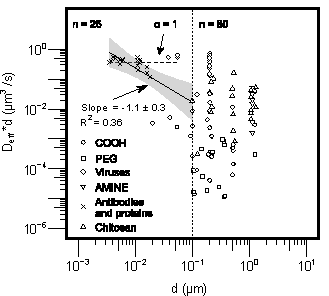
\includegraphics[width = 12 cm]{Figure_SI_diffusion_times_size.pdf}
    \caption{Effective diffusion scaled by particle size. The effective diffusion times the particle size plotted as a function of the anomalous exponent. The solid line represents the regression model. The grey area represents the 95$\%$ confidence interval. Statistically significant slope and $R^2$ of linear regression are displayed. The dashed line shows the trend of particles predicted to display regular diffusion. The legend indicates the symbols associated with each particle type. 
    }
    \label{fig:DiffTimesSize}
\end{figure}

\clearpage

\begin{figure}[H]
    \centering
    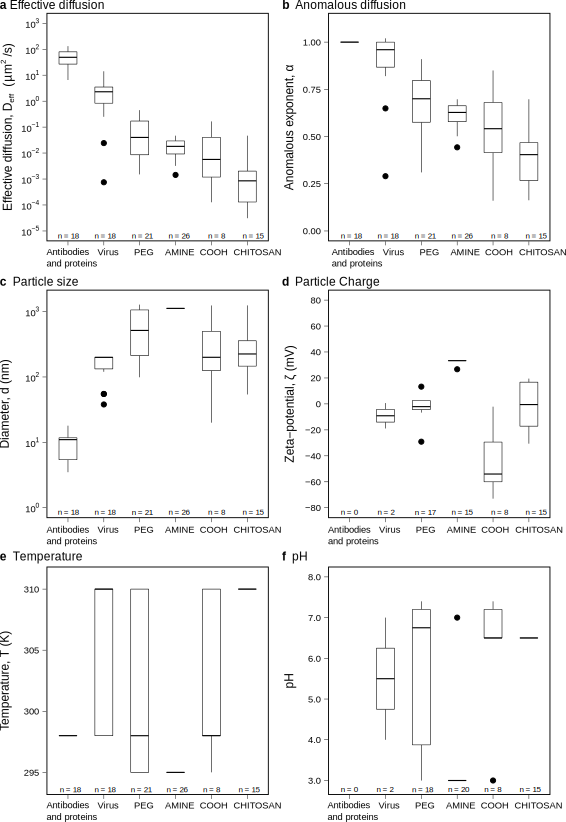
\includegraphics[width = 12 cm]{Figure_Particle_Type.pdf}
    \caption{Transport capabilities based on particle type. \textbf{a},  effective diffusion constant at one second based on particle type \textbf{b}, anomalous exponent based on particle type.  \textbf{c}, .particle size based on particle type. \textbf{d}, particle net charge based on particle type. \textbf{e},  mucus temperature based on particle type. \textbf{f},  mucus pH based on particle type. \textbf{a-f}, box plots are ranked by effective diffusion from high to low. The total amount of data points for each particle type is designated as n aligned with their respected particle type for each panel. 
    }
    \label{fig:ParticleTypeBOX}
\end{figure}

\clearpage

\begin{figure}[H]
    \centering
    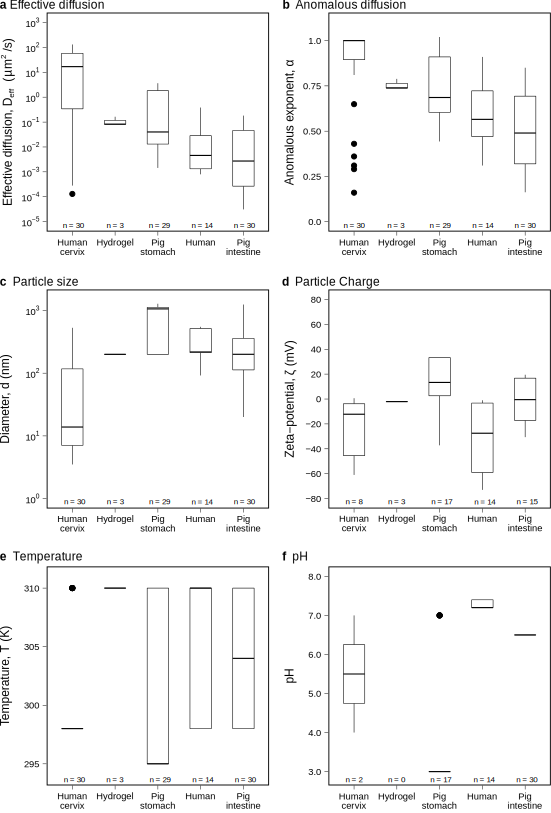
\includegraphics[width = 12 cm]{Figure_Mucus_Source.pdf}
    \caption{Mucus source influence on particle transport.  \textbf{a}, effective diffusion constant at one second based on mucus source. \textbf{b}, anomalous exponent based on mucus source.  \textbf{c},  particle size based on mucus source. \textbf{d}, particle net charge based on mucus source. \textbf{e},  mucus temperature based on mucus source. \textbf{f},  mucus pH based on mucus source. \textbf{a-f}, box plots are ranked by effective diffusion from high to low. The total amount of data points for each mucus source is designated as n aligned with their respected mucus source for each panel.
    }
    \label{fig:MucSourBOX}
\end{figure}

\clearpage

\begin{figure}[H]
    \centering
    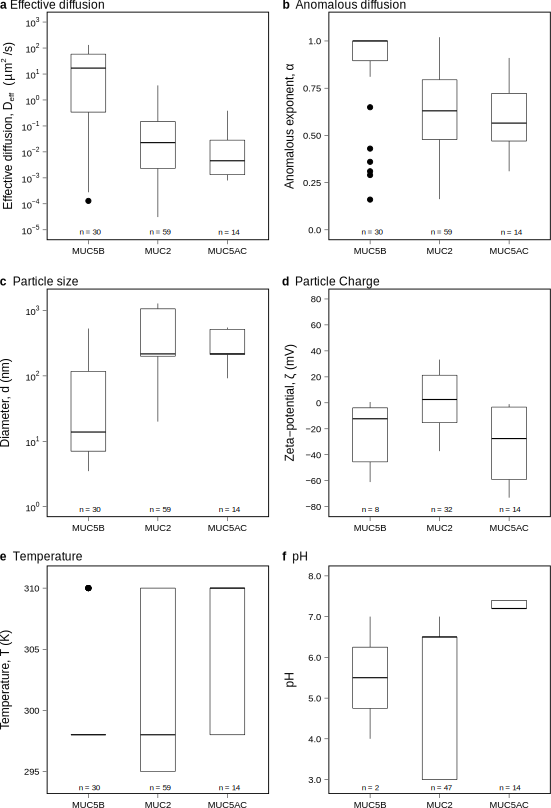
\includegraphics[width = 12 cm]{Figure_Dominant_Mucin.pdf}
    \caption{Impact of dominant mucin genes on particle transport. \textbf{a}, effective diffusion constant at one second based on dominate mucin. \textbf{b}, anomalous exponent based on dominate mucin. \textbf{c}, particle size based on dominate mucin. \textbf{d},  particle net charge based on dominate mucin. \textbf{e}, mucus temperature based on dominate mucin. \textbf{f}, mucus pH based on dominate mucin.  \textbf{a-f}, box plots are ranked by effective diffusion from high to low. The total amount of data points for each dominate mucin is designated as n aligned with their respected dominate mucin for each panel.
    }
    \label{fig:DommucBOX}
\end{figure}

\clearpage

\begin{figure}[H]
    \centering
    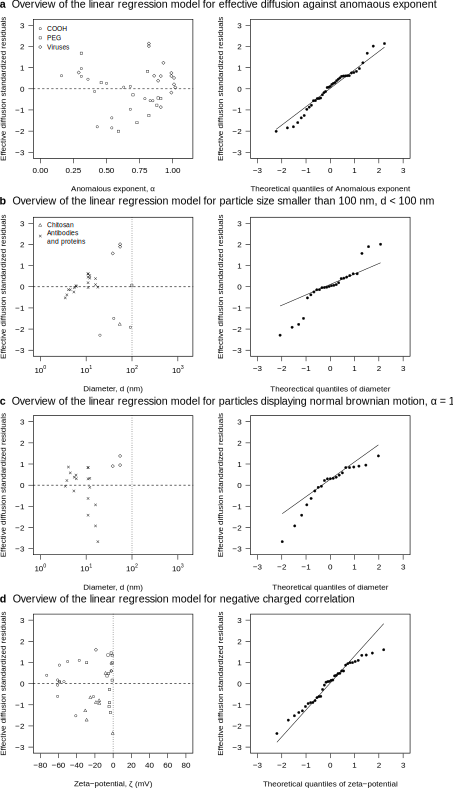
\includegraphics[width = 12 cm]{Figure_Indepth_SLR_analysis.pdf}
    \label{fig:IndepthSLRAna}
\end{figure}

\begin{figure}[H]
    \centering
    \caption{In-depth overview of significant linear regression models. \textbf{a} standardized residuals, and the normal probability of standardized residuals for effective diffusion as a function of the anomalous exponent. \textbf{b} standardized residuals, and the normal probability of standardized residuals for effective diffusion as a function of particle size for sizes less than 100 nm. The dotted line is a visualization marker for particles smaller than 100 nm. \textbf{c} standardized residuals, and the normal probability of standardized residuals for effective diffusion as a function of particle size for particles displaying normal Brownian motion. The dotted line is a visualization marker for particles smaller than 100 nm. \textbf{d} standardized residuals, and the normal probability of standardized residuals for effective diffusion as a function of zeta potential for negatively charged particles. The dotted line is a visualization marker for negatively charged particles. \textbf{a-d}, different particle types with corresponding symbols are designated in \textbf{a} and \textbf{b}'s legend. 
    }
    \label{fig:IndepthSLRAna2}
\end{figure}
 


—
%%%% References %%%%%%%%
%\bibliographystyle{kbib}
%\bibliography{Work}


%%%%% end of supplemenary material %%%%

\end{document}